\documentclass[a4paper,12pt]{amsart}
\usepackage{amsmath}
\usepackage{xcolor}
\usepackage{amssymb}
\usepackage[T1]{fontenc}
\usepackage{tikz}
\usetikzlibrary{patterns}

\begin{document}

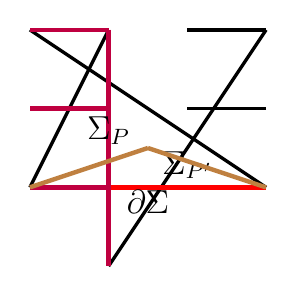
\begin{tikzpicture}[scale=0.5]
\draw [very thick] (-1,-3) -- (-1,3);
\draw [very thick] (-3,-1) -- (3,-1);
\draw [very thick] (-1,-3) -- (3,3);
\draw [very thick] (-3,-1) -- (-1,3);
\draw [very thick] (3,-1) -- (-3,3);
\draw [very thick] (3,-1) -- (1,-1);
\draw [very thick] (3,1) -- (1,1);
\draw [very thick] (3,3) -- (1,3);

\draw [ultra thick,red] (-3,-1)--(-1,-1);
\draw [ultra thick,red] (-1,-1)--(1,-1);
\draw [ultra thick,red] (1,-1)--(3,-1);
\draw [ultra thick,purple] (-1,-1)--(-1,1);
\draw [ultra thick,purple] (-1,1)--(-1,3);
\draw [ultra thick,purple] (-1,-1)--(-3,-1);
\draw [ultra thick,purple] (-1,1)--(-3,1);
\draw [ultra thick,purple] (-1,3)--(-3,3);
\draw [ultra thick,purple] (-1,-1)--(-1,-3);
\draw [ultra thick,purple] (-1,1)--(-1,-1);
\draw [ultra thick,purple] (-1,3)--(-1,-3);
\draw [ultra thick,purple] (-1,1)--(-3,1);
\draw [ultra thick,purple] (-1,3)--(-3,3);
\draw [ultra thick,purple] (-1,1)--(-1,-1);
\draw [ultra thick,purple] (-1,3)--(-1,-3);
\draw [ultra thick,purple] (-1,1)--(-3,1);
\draw [ultra thick,purple] (-1,3)--(-3,3);
\draw [ultra thick,purple] (-1,1)--(-1,-1);
\draw [ultra thick,purple] (-1,3)--(-1,-3);
\draw [ultra thick,purple] (-1,1)--(-3,1);
\draw [ultra thick,purple] (-1,3)--(-3,3);

\node [anchor=south, inner sep=1pt, font=\large] at (-1,0) {$\Sigma_{P}$};
\node [anchor=north, inner sep=1pt, font=\large] at (1,0) {$\Sigma_{P'}$};
\node [anchor=north, inner sep=1pt, font=\large] at (0,-1) {$\partial\Sigma$};

\draw [ultra thick,brown] (0,0)--(-3,-1);
\draw [ultra thick,brown] (0,0)--(3,-1);
\end{tikzpicture}